\documentclass[11pt,a4paper]{article}

\usepackage{main}
\usepackage{evaluation}

\renewcommand{\typedocument}{Évaluation}
\renewcommand{\classe}{5e}
\renewcommand{\titre}{Évaluation 2 -- Electricité (Sujet C)}

\begin{document}

\creertitre{\titre}

\begin{center}
\textit{Durée : 45 minutes -- Calculatrice interdite}
\end{center}

\exercice[4]{Questions de cours}

\question[1]{Donner la définition d'un court-circuit.}

\textbf{Recopier} et \textbf{compléter} les phrases suivantes :

\question[1]{Lorsque le circuit est ouvert, le courant \makebox[2.5cm]{\dotfill} circuler. (peut/ne peut pas)}

\question[1]{Un circuit est dit \makebox[2.5cm]{\dotfill}\ lorsque les dipôles sont reliés les uns aux bornes des autres.}

\question[1]{Le métal est un matériau \makebox[2.5cm]{\dotfill}, il \makebox[2.5cm]{\dotfill} le courant électrique.}

\exercice[3]{Schémas de dipôles}

\textbf{Schématiser} les dipôles suivants :
\vspace*{-0.1em}
\begin{enumerate}
    \item Un générateur
    \item Un interrupteur fermé
    \item Une lampe
\end{enumerate}

\exercice[4]{Schémas de circuits}

Indiquer parmis les schémas 1, 2, 3 et 4, lequel correspond au circuit A et lequel correspond au circuit B.

\vspace{0.1em}

\begin{center}
\begin{tabular}{cc}
    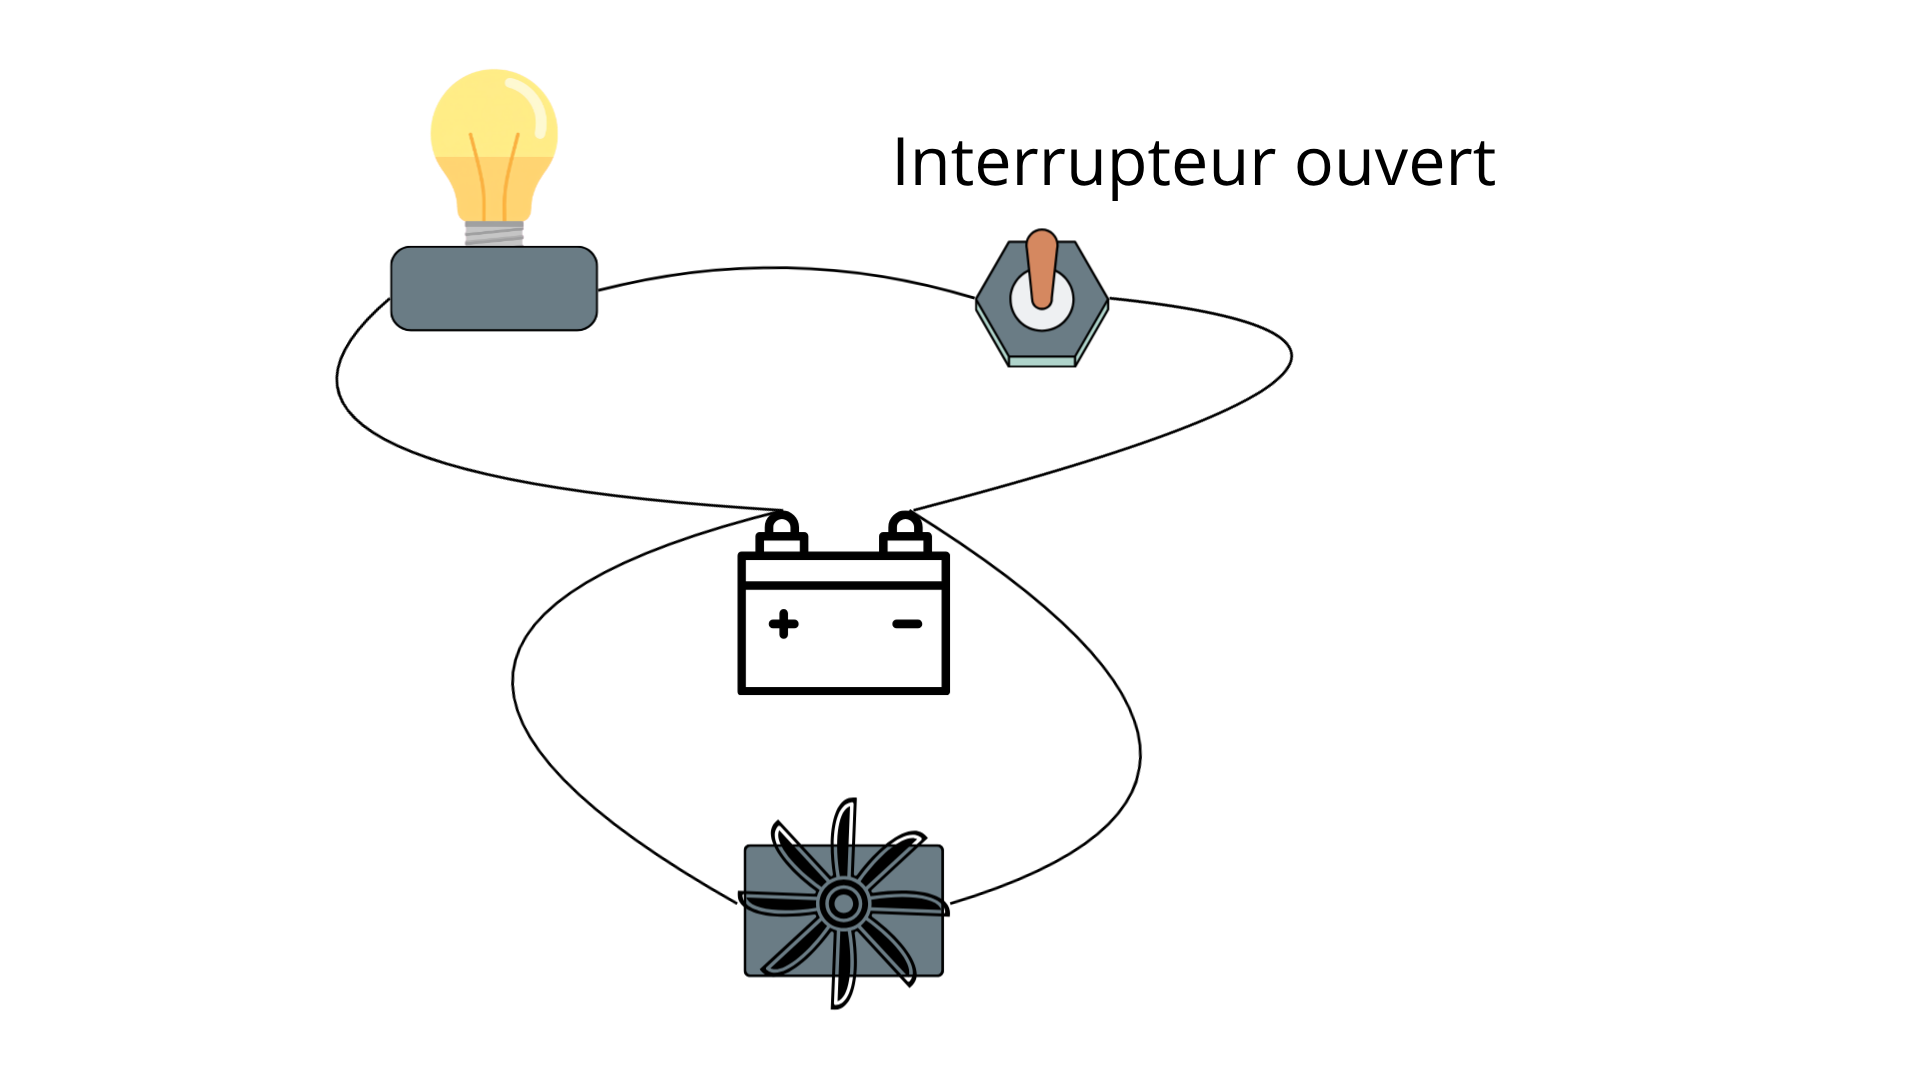
\includegraphics[width=0.4\textwidth]{images/B3a.png} &
    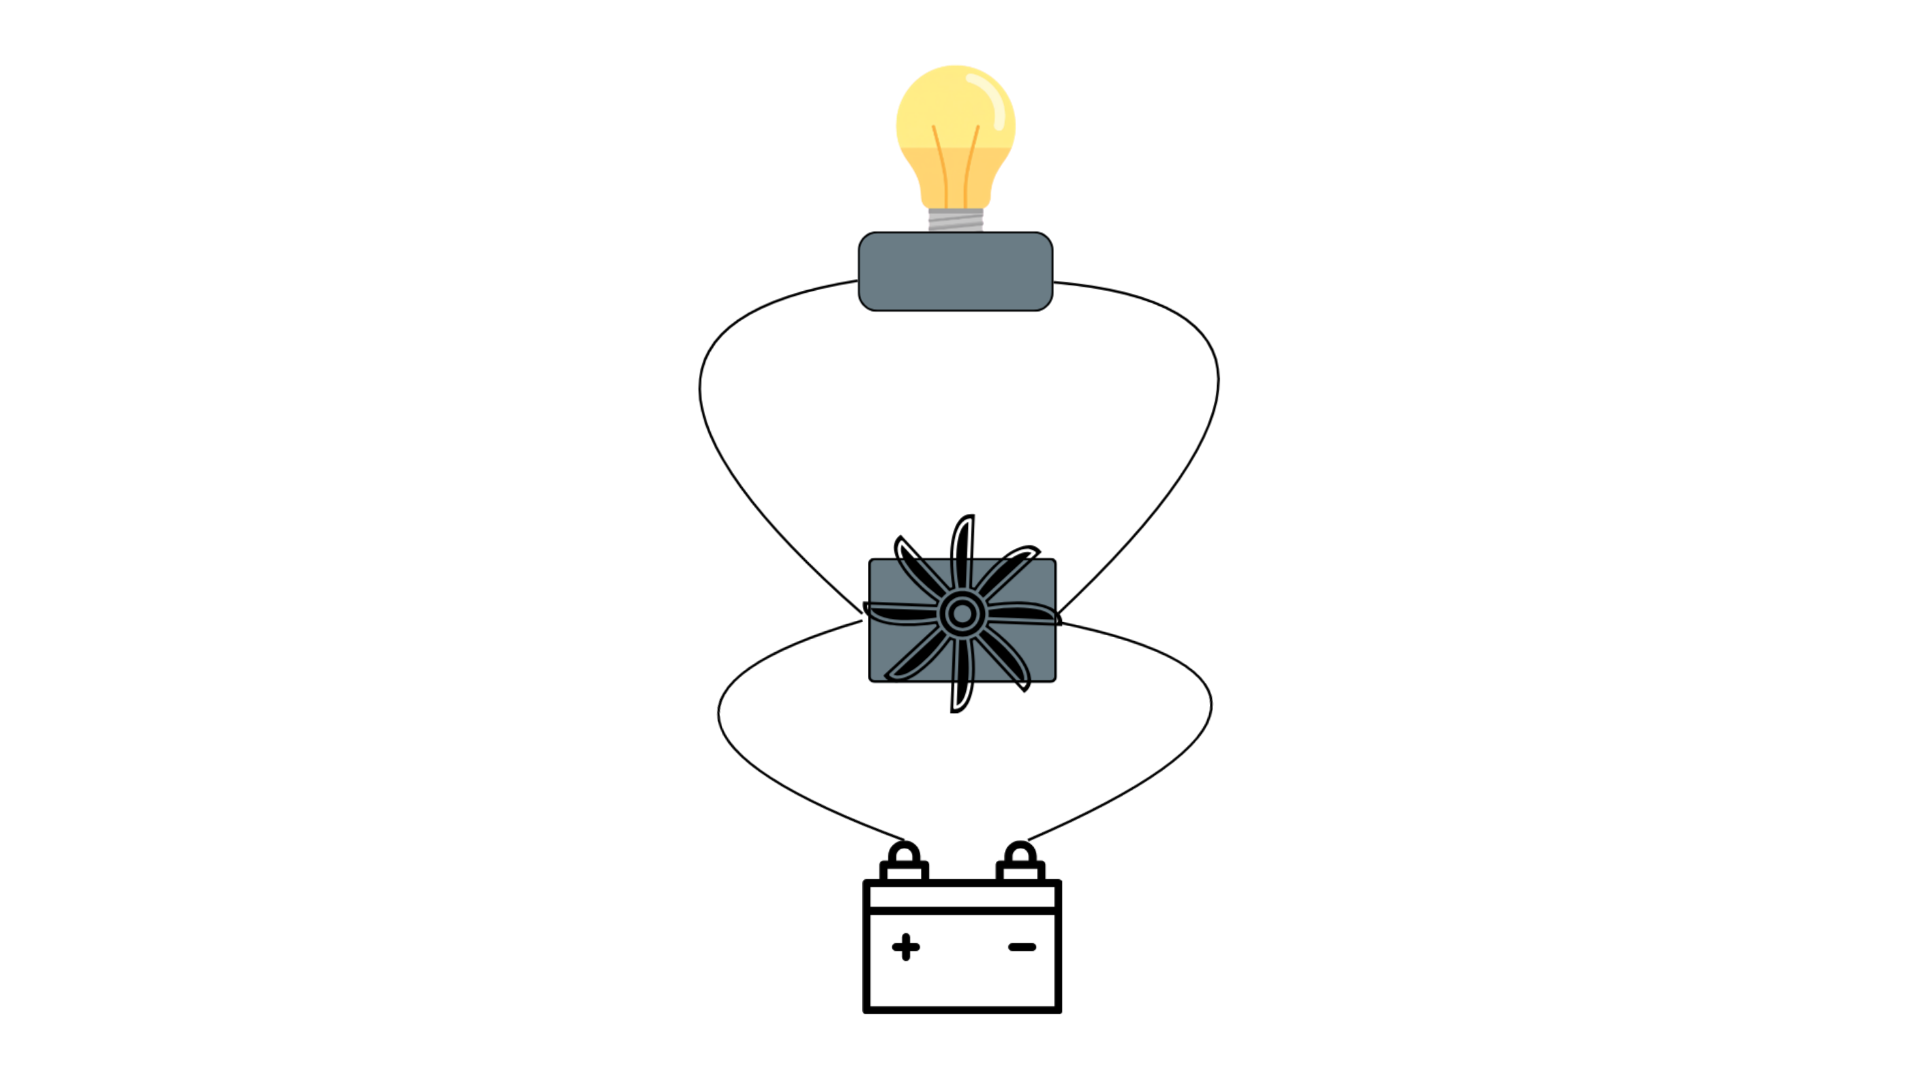
\includegraphics[width=0.4\textwidth]{images/B3b.png} \\
    Circuit A & Circuit B
\end{tabular}
\end{center}

\vspace{0.1em}

\begin{center}
    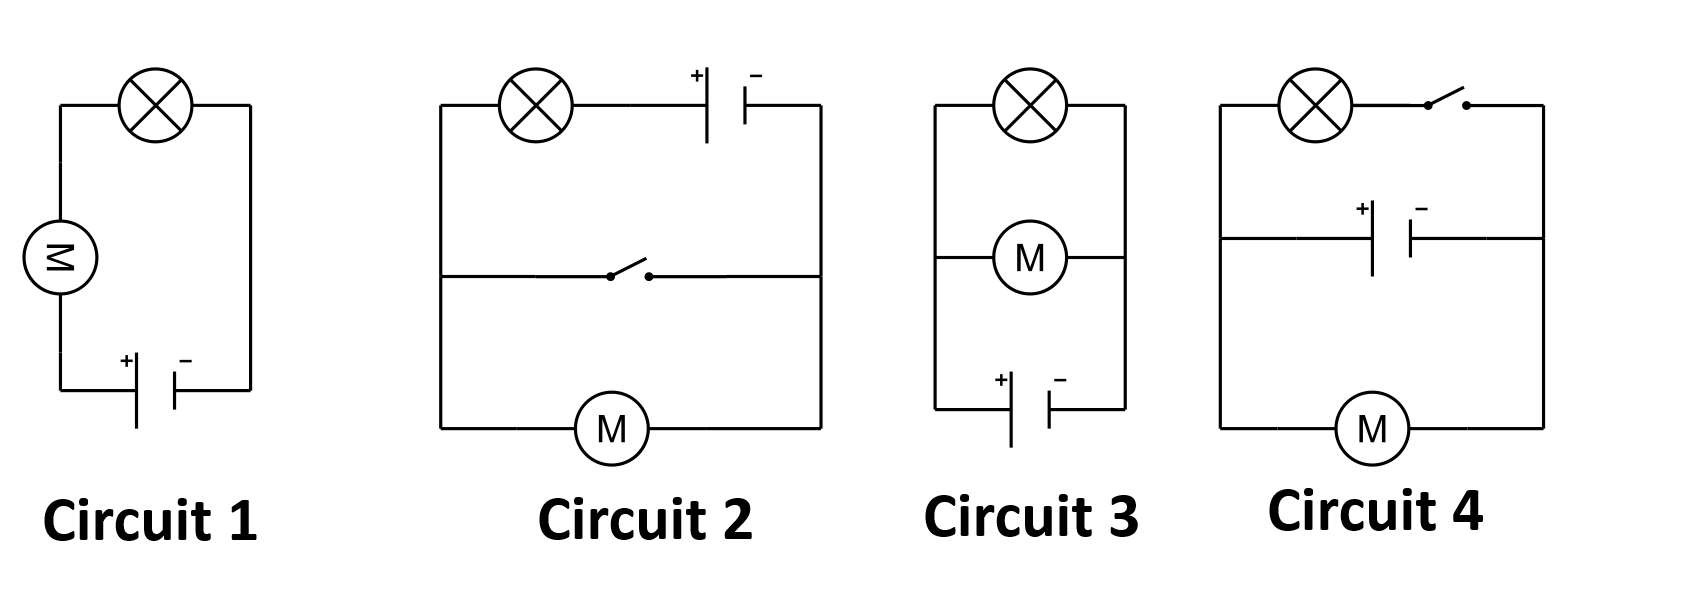
\includegraphics[width=0.8\textwidth]{images/C3.png} \\
\end{center}


\newpage

\exercice[6]{Circuits électriques}

Dans chacun des circuits suivants, \textbf{indiquer} quel(s) dipôle(s) ne fonctionne(nt) pas et \textbf{expliquer} pourquoi.

\begin{center}
\begin{tabular}{cc}
    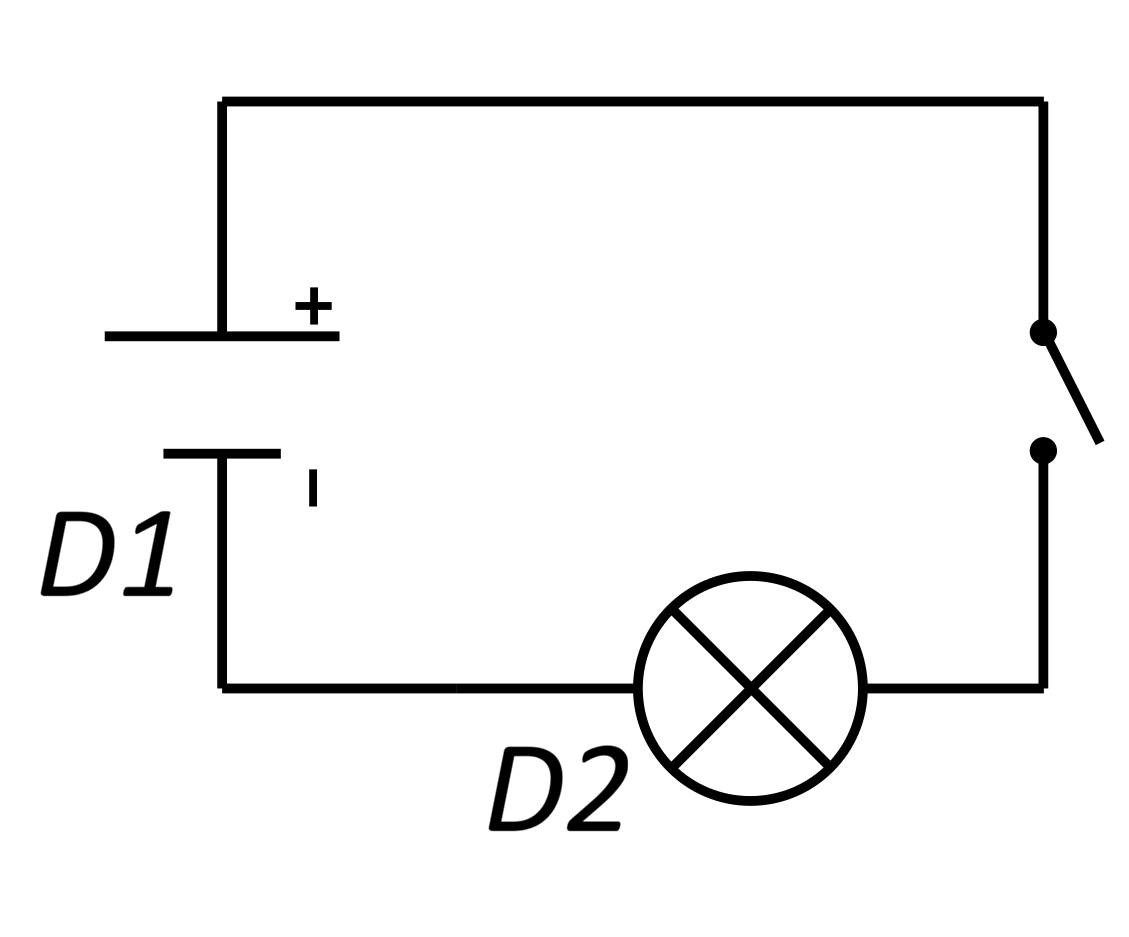
\includegraphics[width=0.2\textwidth]{images/B4a.png} &
    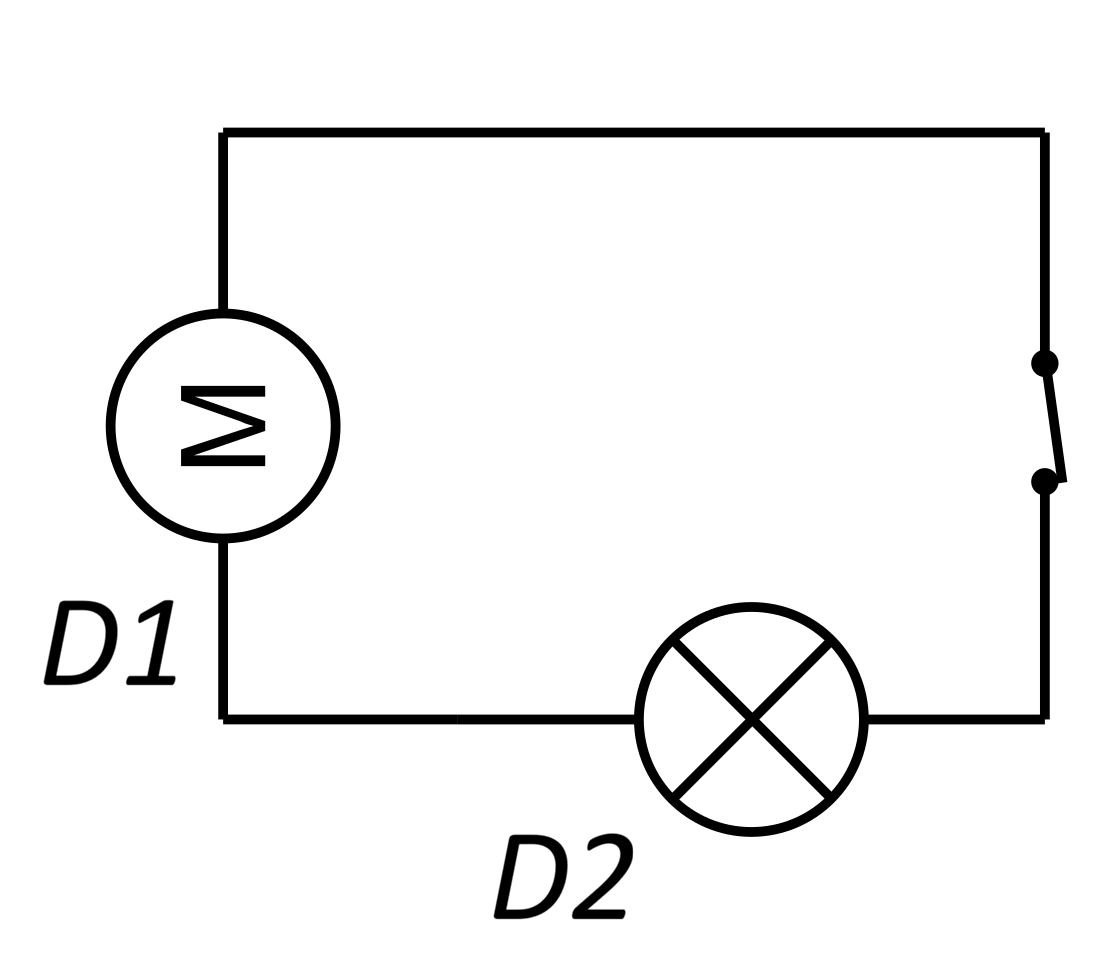
\includegraphics[width=0.2\textwidth]{images/B4b.png} \\
    Circuit A & Circuit B \\
    
\includegraphics[width=0.4\textwidth]{images/4c.png} &
    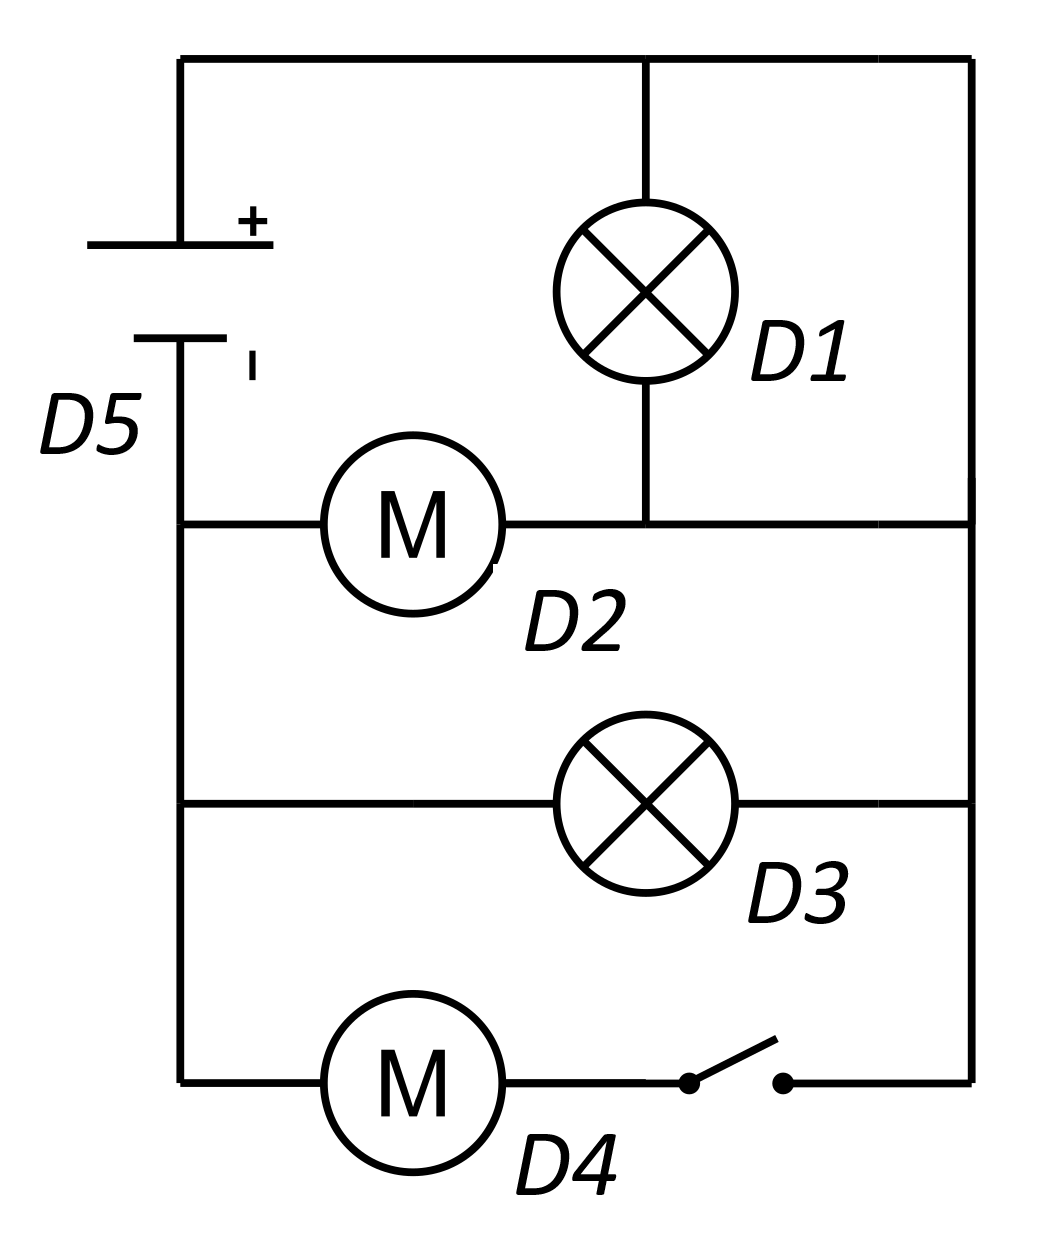
\includegraphics[width=0.25\textwidth]{images/B4d.png} \\
    Circuit C & Circuit D
\end{tabular}
\end{center}

\exercice[3]{Circuit en dérivation}

\begin{center}
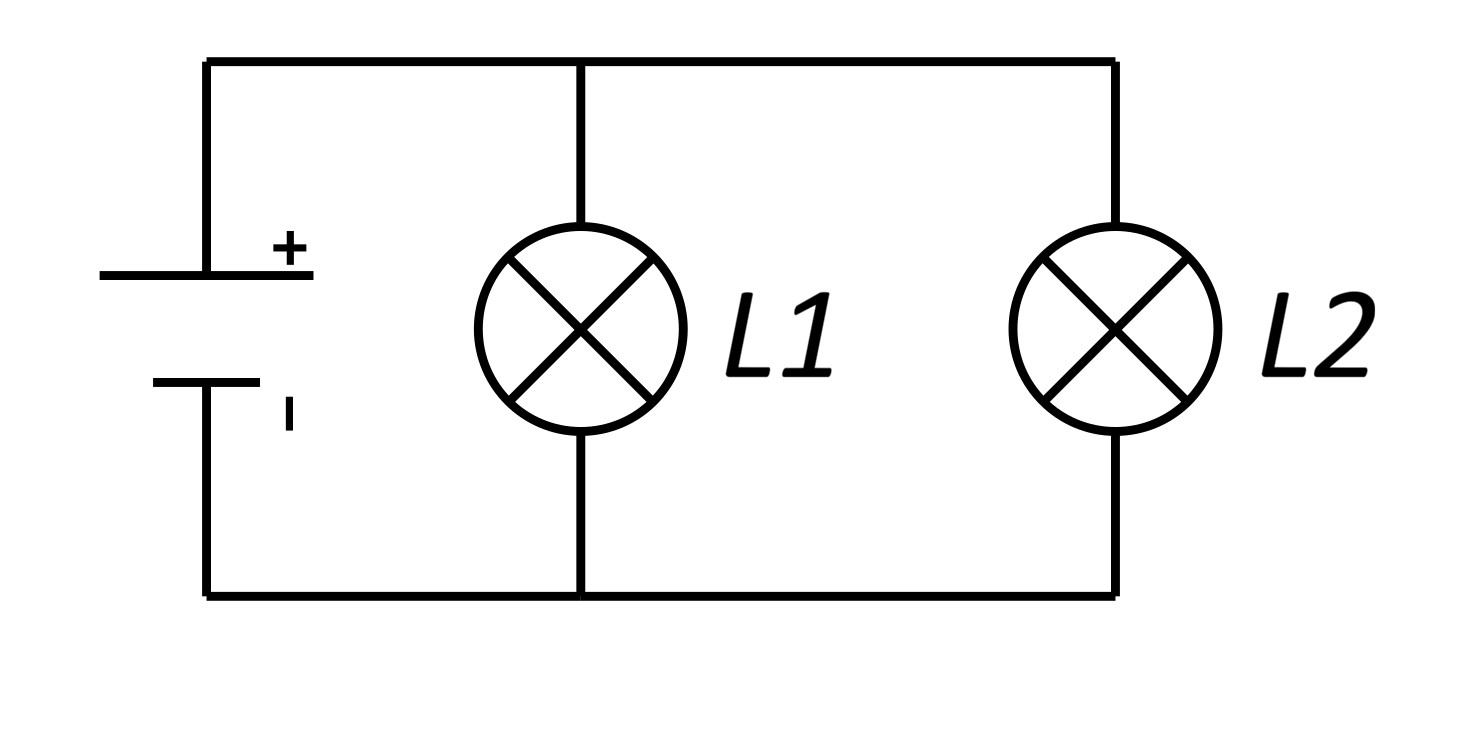
\includegraphics[width=0.5\textwidth]{images/B5.png}
\end{center}

\question[1.5]{Indiquer l'effet sur L2 si L1 est dévissée.}
\question[1.5]{Indiquer l'effet sur L2 si un fil est branché aux bornes de L1.}

\end{document}